\chapter{Generting Unit Tests from a UML Activity}
Our approach for automated generation of test data is based on mathematical programming and the approach for finding relevant control flow paths is based on a simple breadth first search with early infeasible path recognition. Alternatively we can also use depth first search.
%in this Chapter I am going to describe everything I Implemented in the tool as well as some Features I wanted to implement but did not have enough time for.
\section{Generel Overwiew over the Workflow}
The transformation from an UML activity to a CPP Unit test code is divided in five steps. In a first step, the Normalization, where we can check some design rules and parse all embedded OCL constraints and map only the relevant parts from the UML Model onto a simplified meta model of an Activity. The next step is the generation of a mathematical program out of our simplified test model. We are using the AMPL language for that. The third step is a path search where we can find all control flow paths or  those that are necessary to fulfil some coverage criterion of choice. In the fourth step of solving the mathematical program we need to encode a control flow path for which to generate test data in the data for our mathematical program and select a suitable solver to solve the program. In a last step we take the generated solution to the mathematical program and put the values in place within compilable and executable C++ Unit test code. An overview over the complete workflow of our approach is given in figure\ref{fig:workflowOverview}. When infeasible paths need to be detected already during the search of control flow paths the third and fourth step are interfering with each other.
\begin{figure}
\includegraphics[width=\textwidth]{pics/workflow.pdf}
\label{fig:workflowOverview}
\caption{Overview over the Unit Test generation workflow}
\end{figure}
%1.Normalize Model, 2.Make model mathematical Rigurous, 3. Search for Control flow Paths. 4 Solve Mathematical Program for the found Control flow Paths to generate specific Input and output Data. 5. Generate Unit Tests
\section{Normalisation}

\subsection{Design Rules for UML Model} %Structural Design rules
\subsubsection{structural Design Rules}
For our test generation we do assume some design rules to be applied during modelling. The \UMLType{Activity} we generate tests from is an \UMLReference{ownedActivity} of a \UMLType{Class}. The  \UMLType{Class} containing the Activity itself is contained by a \UMLType{Package} or \UMLType{Model}. 
There is an \UMLType{Operation} specifying the \UMLType{Activity}. This \emph{specifying Operation} is either a direct sibling in the UML tree structure and has the same name as the Activity or is explicitly specified by the \UMLReference{specification} reference of the Activity. The specifying Operation will be needed when parsing OCL constraints in section \ref{sec:OCLParsing}.
In figure\ref{fig:StructureExample} we see a tree view of an UML model where those requirements are met.
\begin{figure}
\label{fig:StructureExample}
\includegraphics[width=\textwidht, height=0.5*\textwidth]{}
\caption{Example of a valid structured Model}
\end{figure}
\subsubsection{OCL design rules}
Further we assume that the embedded OCL constraints are either contained within a \UMLType{LiteralString} Element or an \UMLType{OpaqueExpression} with the according Language value set to "OCL". We support a strict subset of the OCL language. The BNF of the supported OCL subset is shown here.

BNF
IntegerLiteral\\
BooleanLiteral: true | false\\
RealLiteral\\
IntVariable\\
RealVariable\\
BoolVariable\\
Number: IntegerLiteral | RealLiteral | IntVariable | RealVariable | ArithmeticOperation\\
ArithmeticOpSymbol: + - * /\\
ArithmeticOperation: Number ArithmeticOpSymbol Number \\
RelationOpSymbol: < | > | <= | >= | = | <> 

RelationOperation: Number RelationOpSymbol Number \\
LogicalOpSymbol: and | or \\
LogicalOperation: Bool LogicalOpSymbol Bool \\

\subsection{A Meta Model suitable for automated Unit Test Generation}
The developed unit test generation algorithm does not work directly on an UML Model but on an ActivityTestCaseGraph. The ActivityTestCaseGraph contains only those details from the UML Metamodel that are really necessary for the test generation. Since it only contains ready parsed OCL Expressions as abstract syntax trees it is much more suitable for the transformation into a mathematical program. \\
The ActivityTestCaseGraph is defined as an extension of a more general AbstractTestCaseGraph model. The AbstractTestCaseGraph meta model was taylored to fit Activities as well as UML \UMLType{Statemachines} in order to be able to apply algorithms not only to Activities but also to \UMLType{StateMachines} as well as to be able to reuse existing Algorithms from ParTeG for \UMLType{StateMachines} for \UMLType{Activities}.

%????
%Figure \ref{fig:ATCGMetamodel} shows the complete meta model of the ActivityTestCaseGraph including all components from the AbstractTestCaseGraph.
%\begin{figure}
%\includegraphics[width=\textwidth]{./pics/ATCGMetamodel.pdf}
%\label{fig:ATCGMetamodel} 
%\caption{Complete meta model of ActivityTestCaseGraph}
%\end{figure}
%????

\subsubsection{Abstract Test Case Graph}

\begin{figure}
\label{fig:AbstractTCGMetaModel}
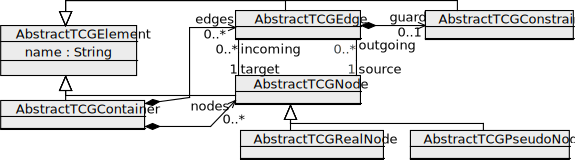
\includegraphics[width=0.5\textwidth]{./pics/AbstractTestCaseGraph.pdf}
\caption{Meta model of the AbstractTestCaseGraph}
\end{figure}
An Abstract Test Case Graph is a directed graph consisting of nodes (AbstractTCGNode) and edges (AbstractTCGEdge). Each edge has source and a target node. Each node can have multiple outgoing and multiple incoming edges.
A node can either be a pseudo node (AbstractTCGPseudoNode) or a real node (AbstractTCGRealNode). A pseudo node is a node that you can insert in the middle of an edge without changing any of the semantics of the test model. Edges can have a guard condition of type AbstractTCGConstraint. Such a graph is contained by a Container (AbstractTCGContainer). The container has a singular reference to one of its owned nodes declaring this as the initial node. \\
The semantics of the activity test case graph is Petri net like. When executing a test case graph we have at the beginning a token in the initial node that can move along the edges. The token can only move along an edge, when its guard condition is true. When an token resides in a node we say that the node is executed.

\subsubsection{Activity Test Case Graph}
\begin{figure}
\label{fig:ActivityTCGMetaModel}
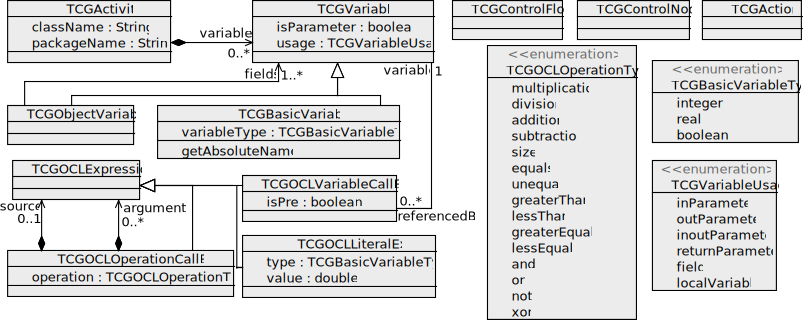
\includegraphics[width=\textwidth]{./pics/ActivityTestCaseGraph.pdf}
\caption{Meta model of the ActivityTestCaseGraph}
\end{figure}
An activity test case graph is an extension to the abstract test case graph especially tailored for test generation from activities. The activity test case graph models control flow and constraints on variables that need to hold at different points during execution of the activity test case graph. Its Metamodel is shown in figure\ref{fig:ActivityTCGMetaModel}.\\
The TCGActivity is an extension of the AbstractTCGContainer. As well as TCGAction, TCGControlNode and TCGControlFlow do refine the types AbstractTCGRealNode, AbstractTCGPseudoNode and AbstractTCGEdge respectively. 
The main extensions to the abstract meta model are the Variables and the elements of an abstract syntax tree to express constraints and the TCGAction.
\paragraph{TCGAction} A TCGAction can in addition to its supertye contain arbitrary many localPostconditions of the type AbstractTCGConstraint. A local Postcondition has the semantic, that it has to be true after the execution of the action. This implies changing some variables throughout the execution of the action.
\paragraph{OCL Abstract Syntax Tree}

TCGOCLExpression is a subtype of AbstractTCGConstraint. A TCGOCLexpression can either be an Operatiton call with a source and  arguments or a TCGOCLLiteralExpression holding a literal value and its data type or a TCGOCLVariableCallExp referencing a TCGVariable. The isPre attribute of TCGOCLVariableCallExp denotes whether in the original OCL expression has been an "@pre" with the token. TCGOCLExpression and its subtypes do form a simplified OCL abstract syntax tree.
\paragraph{Variables}
A TCGVariable can be one of two subtypes either a TCGBasicVariable or a TCGObjectVariable. An object variable is put together by one or more other variables. A basic variable has one of the three variableTypes that can be handled by our approach: Integer, Real, Boolean. A TCGVariable is a place holder for a value. When the isParameter field is true it can only hold one Value throughout the execution of the TCGActivity otherwise it can change its value during each execution of an TCGAction.

\subsection{Transforming UML to ActivityTestCaseGraph}
An Instance of the activity test case graph meta model serves as a normalized input model. We use a model to model transformation to transform an \UMLType{Activity} from a UML Model into an activity test case graph. In many cases the transformation is straight forward: for one Element in the UML model the corresponding element in the activity test case graph is produced. When one element of the UML model is mapped to one Element of the activity test case graph model we call the uml element \emph{source element} and the created element in the activity test case graph model \emph{target element}.
\subsubsection{Mapping UML Elements to Activity Test Case Graph Elements}
\begin{figure}
\label{fig:UML2TCGTranformation}
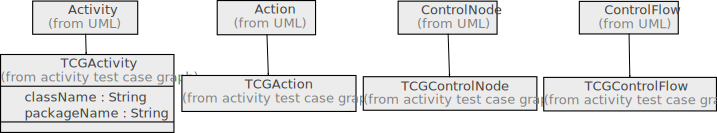
\includegraphics[width=0.6\textwidth]{./pics/UML2TCGTransformation.pdf}
\caption{UML elements being mapped straight forward to activity test case graph elements}
\end{figure}

\paragraph{Activity}
A UML Activity is transformed into a TCGActivity. For the test generation process described in section \ref{sec:UnitTestGen} we need to store the name of the containing class of the Activity as well as the full pathname to the package containig this class in the property fields of the TCGActivity. For each activity all of its ownedNodes as well as ownedEdges are considered for transformation.
\paragraph{Action} Those ownedNodes of the Activity that are a subtype of Action transformed into a TCGAction. To specify the behaviour of the TCGAction localPostconditions are considered for transformation. The detailed semantics of special subtypes of an Action are neglected.
\paragraph{ControlNode}OwnedNodes that are a subtype of ControlNode are transformed into TCGControlNodes. That means they are pseudo nodes. It is assumed that there is only one UML InitialNode. Its corresponding TCGControlNode is referenced by the TCGActivity as initial node.
\paragraph{ControllFlow} Out of the ownedEdges of the \UMLType{Activity} we transform the \UMLType{ControlFlows} into TCGControlFlows. If there is a guard condition this is handled like a constraint.

\subsubsection{parsing OCL Constraints}
\UMLType{Constraints}, and \UMLType{Properties}, as well as \UMLType{Parameters} can not be transformed straight forward. We parse the textual OCL expression contained in a \UMLType{Constraint}, or the \UMLReference{guard} attribute of a \UMLType{ControlFlow}. When the OCL expression was parsed correctly we have an abstract syntax tree of this expression. The elements of this abstract syntax tree will be transformed to TCGOCLExpression elements and all \UMLType{Properties} and \UMLType{Parameters} referenced by the OCL abstract syntax tree will be transformed into TCGVariables. We ensure, that only those OCL expressions are in the activity test case graph that later on can be transformed into an AMPL model as explained in in section \ref{sec:AmplModelling}. We also ensure that our CSP that we will formulate with AMPL will only contain variables that are constraint by at least one constraint. There might be properties of a class that are not changed by an operation and whose value do not have any influence on the control flow in the implementation of this operation. A variable representing such an irrelevant property will not appear in the rigorous model.
\paragraph{Extracting textual OCL}
Textual OCL expressions are contained within \UMLType{Constraints} as explained in section \ref{sec:Constraint}. When the Constraint contains a \UMLType{LiteralString} we will try to parse its \UMLReference{value} as OCL. If the \UMLType{Constraint} contains an \UMLType{Opaque Expression} we will first check whether the \UMLReference{language} attribute contains the value "OCL" and try to parse the corresponding value of the \UMLReference{body} attribute. If the \UMLReference{language} attribute does not contain the value "OCL" then we will try to parse the concatenation of all \UMLReference{body} values of the \UMLType{OpaqueExpression}.\\ The \UMLReference{guard} of a \UMLType{ControlFlow} can also contain a \UMLType{LiteralString} or an \UMLType{OpaqueExpression}. The extraction of textual OCL from a \UMLType{ControlFlow} is analogue to the extraction from a Constraint.
\paragraph{parsing textual OCL}
\label{sec:OCLParsing}
Details of the OCL have been explained in \ref{sec:Constraint}. For this thesis we consider three types of constraints: \emph{invariants}, \emph{postconditions} and \emph{guard conditions}. Every OCL constraint is parsed with respect to a \emph{context}. The context resolves the variables referenced within the OCL expression. For Example the "self" keyword always returns the instance for which the constraint is evaluated.\\
Textual OCL found inside a \UMLType{Constraint} contained by the \UMLReference{ownedRule} reference of either the \UMLType{Activity} or its containing \UMLType{Class} will be interpreted as invariant. Invariants need to be true before the \UMLType{Activity} is executed, throughout its execution, and after the execution of the \UMLType{Activity} has finished. We are parsing the invariants according to the OCL specification as invariants of the specifying \UMLType{Operation}. \\
The OCL expressions found within \UMLReference{guards} of \UMLType{ControllFlows} will also be parsed as if they were an invariant of the specifying \UMLType{Operation}.
That means for guards and invariants all attributes of the \UMLType{Class} as well as all \UMLReference{ownedParameters} of the specifying \UMLType{Operation}, and all properties of the containing \UMLType{Packages} are accessible.\\
\UMLType{Actions} can also contain multiple \UMLType{Constraints} within their \UMLReference{localPostcondition} reference. Any textual OCL found within a \UMLReference{localPostcondition} will be parsed as postcondition in the context of the specifying \UMLType{Operation}. All variables accessible for guards and invariants are also accessible for postconditions. Only in postconditions the OCL "@pre" is allowed. Postconditions are required to hold after the execution of the \UMLType{Action} they belong to. With "@pre" we refer to the value of a variable before the execution of the \UMLType{Action}.

\paragraph{Transforming the Abstract Syntax Tree}
\begin{figure}
\includegraphics[width=\textwidth]{}
\end{figure}
If the OCL parser was supplied with a valid OCL expression for the context that was assumed then it will return an abstract syntax tree for the parsed OCL expression. We are interested in a subset of the OCL abstract syntax trees. 

\paragraph{transforming Properties and Parameters}
whenever the OCL abstract syntax tree containes a property call or a variable reference then the referenced \UMLType{Property} or \UMLType{Parameter} will be transformed into a TCGVariable. All TCGVariables are contained by the variables reference of the root element of the activity graph, the TCGActivity.\\
For \UMLType{Parameters} and \UMLType{Properties} we need to check their \UMLReference{type} reference. If the name of the \UMLType{Type} is one out of a list of names that can be mapped to either Integer, Real or Boolean then a TCGBasicVariable is created for it and its variableType field set accordingly to one out of Integer, Real or Boolean. The exact mapping of names of the \UMLType{Type} to a TCGvariableType is implementation specific. One could for example map from "uint32\_ t" to Integer.\\
If a \UMLType{Parameter} was transformed into a TCGBasicVariable then the isParameter field is set to true, indicating that this Variable has been a \UMLType{Parameter}. For \UMLType{Properties} the isParameter field of the resulting TCGBasicVariable will be set to false.\\
The field usage of the the TCGBasicVariable can take values from the enumeration TCGVariableUsage. This information will be needed when creating the c or c++ unit tests as described in section \ref{sec:UnitTestGeneration}. If the TCGBasicVariable was created to represent a Parameter it could have been an input parameter, an output parameter, an inout parameter, or a return parameter. The value of the usage field for a transformed \UMLType{Parameter} is determined by the value of the \UMLReference{direction} field of the original \UMLType{Parameter}.


%according to the OCL specification as explained in section \ref{sec:OCL}. 

 When the textual expression was successfully parsed according to the OCL specification we hold an abstract syntax tree of the OCL Expression as explained in \ref{sec:OCL}. The elements from the OCL abstract syntax tree are then transformed into TCGOCLExpressions. Whenever a 
transform then only those \UMLType{Properties} and \UMLType{Parameters} into TCGVariables, that are referenced in the parsed OCL Expressions.\\ 

A UML Constraint can be specified in several ways e.g as StringLiteral or as OpaqueExpression. It is depending on the used modelling tool how the textual OCL is saved in the Model. We are extracting the textual OCL Expressions and parse them according to the OCL specifications. If they can not be parsed the extracted text was either not an OCL expression or it is a faulty one. In those cases this constraint will be ignored.

The transformation ensures that every TCGOCLConstraint has a globally unique name. This is not always the case in the original UML model.

\subsection{Further Model 2 Model Transformations}
\subsubsection{Removing logical operations}
%\subsubsection{
\subsubsection{Handling Structured Activity Nodes}
\subsubsection{Mapping self defined Datatypes to standard Types}
Explain the ActivityTestCaseGraph Metamodel and the transformation from UML with embedded OCL to it. 
suggest a few further M2M transformations to make the model easier to digest for the actual test generation.
\section{AMPL Modeling}
Tell about the AMPL Modelling i.e. variables are becoming arrays to hold one initial Value and for each TCGAction on the Path one that makes its postconditions and general Invariants valid. One specific control flow Path is encoded in the AMPL data, so we can take advantage of the interactive solving capabilities of AMPL and the connected solvers.
By adding an objective Function to the AMPL Model after any solution has been found it is extremely easy to get boundary Values for testing.
\subsection{Transforming Variables and Parameters}
\subsection{Transforming LocalPostConditions, Guards and Invariants}
\subsection{Specifying Control Flow Paths in the AMPL Data}
\subsection{Generate Boundary Values}
\section{Pathsearch}
Bounded BFS, and Bounded DFS, and DFS with early infeasible Path elimination.
Suggest to extend the search algorithms to work with test goals as explained by Stephan Weißleder.
\subsection{Depth First Search}
\subsection{Breadth First Search}
\subsection{Early Infeasible Path Elimination}
This feature can also be used to specify for loops an upper bound of iterations as well as a lower bound of loop iterations to test. You just need to add some guard conditions in front of the loop referencing the loop variant.
\subsection{Generating Unit Tests}
\label{sec:UnitTestGeneration}
\label{sec:UnitTestGen}
\section{Implementation}
say a few words about EMF and Eclipse Plugin. Tell that I used Eclipse org.eclipse.ocl.uml and eclipse org.eclipse.uml2.uml packages. //Could potentially also move to preliminaries
\subsection{The Eclipse Modelling Framework}
\cite{EMF}
\subsubsection{Importing Models from Atego Artisan Studio}
\subsubsection{Model transformations}
\subsubsection{Parsing OCL Expressions}
\subsection{Using the resulting Plugin}
